\documentclass[10pt,journal,final,finalsubmission,twocolumn]{IEEEtran}
%\pagestyle{empty}
%\documentclass[9.5pt,journal,final,finalsubmission,twocolumn]{IEEEtran}
%%%%%%%%\renewcommand{\baselinestretch}{2}
\usepackage{stmaryrd}
\usepackage{amsfonts}
\usepackage{url}
\usepackage{mathrsfs,amsmath}
%\usepackage{caption2} 
\usepackage{graphicx,times}
\usepackage{cleveref}
\usepackage{cite}
\usepackage{amssymb}
\usepackage{makeidx}
\usepackage{multirow}
\usepackage{subfigure}
\usepackage{algorithmic} 
%\usepackage{ntheorem}
%\usepackage[justification=centering]{caption}
\usepackage{bm}
\usepackage[ruled,linesnumbered,vlined]{algorithm2e}  
%\usepackage{caption}
%\usepackage[top=2cm, bottom=2cm, left=2cm, right=2cm]{geometry}    
\usepackage{setspace}
\usepackage{amsthm}
\usepackage{booktabs}
\usepackage{authblk}



\newtheorem{theorem}{Theorem}
\newtheorem{lemma}[theorem]{Lemma}
\newtheorem{proposition}{Proposition}
\newtheorem{definition}{Definition}
\newtheorem{corollary}[theorem]{Corollary}
\newtheorem*{pf}{Proof}


%\newenvironment{proof}{{\noindent\it Proof}\quad}{\hfill $\square$\par}



\newcommand{\tabincell}[2]{\begin{tabular}{@{}#1@{}}#2\end{tabular}}
% correct bad hyphenation here
\hyphenation{}
\IEEEoverridecommandlockouts    % to create the author's affliation portion
                % using \thanks

%\textwidth 178mm    % <------ These are the adjustments we made 10/18/2005
%\textheight 239mm   % You may or may not need to adjust these numbes again
%\oddsidemargin -7mm
%\evensidemargin -7mm
%\topmargin -6mm
%\columnsep 5mm
\renewcommand\thepage{}
%\renewcommand{\baselinestretch}{1.57}
\allowdisplaybreaks

\begin{document}

\title{Leveraging Muiti-cell NOMA for Cell Edge}

\author{Zhanwei Yu\textsuperscript{1}, Lei You\textsuperscript{2} and Di Yuan\textsuperscript{1}}
\affil{\textsuperscript{1}Department of Information Technology, Uppsala University, Sweden
\authorcr \textsuperscript{2}Independent Researcher, Sweden
\authorcr {\em Emails: zwyuapr1@gmail.com;lei.you@pm.me;di.yuan@it.uu.se}}
\renewcommand*{\Affilfont}{\small}

\maketitle
\begin{abstract}
Non-orthogonal multiple access (NOMA) is a promising 
technique for performance enhancement in cellular networks. This paper investigates how much NOMA can offer for cell edge in multi-cell scenarios. We consider the joint optimization problem of time-frequency resource allocation, user pairing, and power split, for scaling up the demand delivered for edge users. Our approach for problem solving consists in iteratively applying a fixed-point method to the cells, and, for each cell, deriving an algorithm guaranteeing optimum for single-cell optimization. By embedding  the fixed-point method into bi-section search, we are able to show the overall approach guarantees global optimality. Numerical results demonstrate that multi-cell NOMA optimization has much more to offer over orthogonal multiple access for the experience of edge users, in particular for high-demand and resource-limited scenarios. 
\end{abstract}


\begin{keywords}
NOMA, multi-cell, cell edge, resource allocation
\end{keywords}

%-----------------------------------------------------------------------------------------------------------------------------------------------
\section{Introduction}  \label{Sec:Intro}

Designing beyond-5G systems targets squeezing more bits out of the spectrum. Non-orthogonal multiple access (NOMA) is considered a promising radio access technique for performance enhancement. The basic idea of NOMA is using the same transmission channel to simultaneously serve multiple user equipments (UEs) at the cost of inter-user interference. By utilizing successive interference cancellation (SIC), NOMA can achieve better  performance than orthogonal multiple access (OMA).

The experience of edge UEs is an important performance metric. There are a number of works studying improving this metric with NOMA. In \cite{Do1}, the performance of a single edge UE in a two-user multiple-input single-output (MISO) NOMA system is studied and three cooperative downlink transmission schemes with simultaneous wireless information and power transfer (SWIPT) are proposed. To improve the experience of the edge UEs in a two-user NOMA system, the authors of \cite{Do2} propose two cooperative relaying schemes, called on/off full-duplex relaying and on/off half-duplex relaying. In \cite{Guo}, a two-cell NOMA system is considered, where two center UEs are served by their respective cells and one edge UE is served by both cells, the authors propose both centralized and distributed algorithms to minimize the total transmit power. In \cite{Pei}, the authors propose a downlink NOMA based coordinated direct and relay system with one center UE and multiple edge UEs, where a decode-and-forward and full-duplex relay is used to help the latter.

The works in \cite{Do1, Do2, Guo, Pei} all focus on single-cell or two-cell scenarios. For more general multi-cell NOMA, resource optimization is more challenging, due to the interplay between SIC and inter-cell interference.

Recently, some studies have addressed general-scenario multi-cell NOMA. The authors of \cite{Ali} consider the problem of dynamic power allocation with coordinated multi-point (CoMP) transmission in the downlink and propose a distributed power optimization approach. The authors of \cite{You1} study the cell load coupling system for multi-cell NOMA, and propose an algorithm for power allocation and UE pairing for optimal resource management. A complementary note to \cite{You1} is provided in \cite{You2}. The authors of \cite{Ni} study the total transmit power minimization problem for multi-cell and multi-carrier NOMA (MCMC-NOMA) networks, and propose a resource allocation algorithm which can dramatically reduce the power consumption. The authors of \cite{Lei} investigate energy optimization in MCMC-NOMA networks, and propose tailored algorithms to provide energy-efficient solutions for three NOMA grouping schemes.

Different from \cite{Do1, Do2, Guo, Pei}, which focus on single-cell or two-cell NOMA systems, we consider more general multi-cell scenarios. In addition, we focus on the experience of edge UEs. Indeed, the achievable rate of the edge UEs is generally much lower than that of the cell-center UEs \cite{Dai}. We aim at investigating how much NOMA can offer to edge UEs. To this end, we study the joint optimization problem of time-frequency resource allocation, UE pairing, and power split, with the objective of maximizing the amount of data delivered to cell-edge UEs. We formulate this problem and derive its fundamental properties. We first propose a single-cell algorithm, aiming to minimize time-frequency resource consumption for any given amount of data to be delivered to the edge UEs within one cell, while the resource allocation of other cells is tentatively fixed. Next, we iteratively apply a fixed-point method with the single-cell algorithm to minimize multi-cell resource consumption. Then, we approach the global optimum of the overall problem by embedding the fixed-point method into bi-section search. Finally we evaluate the performance of algorithm in multi-cell NOMA compared to OMA.

%-----------------------------------------------------------------------------------------------------------------------------------------------
\section{System Model and Problem Formulation} \label{Sec:SystemModel}

\subsection{System Model}\label{Preliminaries}

Denote by $\mathcal{I} = \{1,2,...,I \}$ and $\mathcal{J} = \{1,2,...,J\}$ the sets of cells and UEs, respectively. 
We consider downlink and denote by $g_{ij}$ the channel power gain from cell $i$ to UE $j$ $(i \in \mathcal{I}, j \in \mathcal{J})$. Denote by $\mathcal{J}_i$ the set of UEs served by cell $i$.

The time-frequency resource is divided into resource units (RUs). In NOMA, multiple UEs can access the same RU by SIC. However, the complexity of decoding grows rapidly with the number of UEs involved in SIC. It has been demonstrated that two UEs in SIC can offer a good trade-off between complexity and performance \cite{Islam}. In view of this, we consider two UEs in one cell sharing one RU as a {\em pair} (denoted by $u=\{j,h\}$), and call the process of selecting UEs to form pairs as {\em UE pairing} or simply {\em pairing}. To keep the generality, a pair may consist of a single UE $j$, i.e., UE uses the OMA mode, and we denote this special pair by $u=\{0,j\}$. For cell $i$, denote by $\mathcal{U}_i$ the set of all candidate pairs of UEs in $\mathcal{J}_i$. Similarly, use $\mathcal{U}_j$ to refer to the set of all pairs containing UE $j$. Furthermore, we use ${\mathcal{U}}$ to refer to the set of all candidate pairs, i.e., $\mathcal{U} = \bigcup _{i \in \mathcal{I}}  \mathcal{U}_i$, and use $N$ to denote the cardinality of U, i.e., $N=|\mathcal{U}|$. Also, we put indices on $u$ to differentiate between the pairs, i.e., $\mathcal{U} = \{u_1,u_2,...,u_N\}$. We use a binary $y_{u}$ to indicate whether or not the pair $u$ is selected. We optimize pairing by optimizing $\boldsymbol{y}$, where $\boldsymbol{y} = [y_{u_1},y_{u_2},...,y_{u_N}]$.

We use $p_i$ to denote the transmission power of cell $i$ on an RU. For each pair $u$ in cell $i$, {\em power splitting} is done on $p_i$, with $q_{ju}$ and $q_{hu}$ allocated to UE $j$ and $h$, respectively. Namely,
\begin{equation}
p_i = q_{ju} + q_{hu}.
\end{equation}
Besides, denote by $x_u$ the proportion of RUs allocated to pair $u$. We have
 \begin{equation}
 \rho_i = \sum \nolimits_{u \in {\mathcal{U}}_i} x_u \leq \bar{\rho},  i\in \mathcal{I},
 \end{equation}
where $\bar{\rho}$ is how many RUs at most can be allocated in one cell. 

%We remark that we obtain optimal pairs by optimizing $\boldsymbol{x} = [x_{u_1},x_{u_2},...,x_{u_N}]$ and the optimal $\boldsymbol{x}^*$ also represents the result of pairing optimization. If any $x_u^* > 0$, UEs $j$ and $h$ form a pair $u$ to share RU in NOMA mode, and if $x_u^* = 0$, then UEs $j$ and $h$ ($j,h \in u$) do not share RU.

For any UE $j$ $\left(j \in u\right)$, the signal-to-interference and noise ratio (SINR) is computed by
\begin{equation}
\gamma _{ju} \!=\!\frac{q_{ju}g_{ij}}{{B_{ju}q_{hu}g_{ij}}\!+\!{\sum_{k\in \mathcal{I}\setminus \left \{ i \right \}}p_kg_{kj}\rho_k}\!+\!\sigma ^2}, j\!\in\! u, u \!\in\!{\mathcal{U}}.\label{1111}
\end{equation}
We set $\gamma_{0u} = 0$ to for with the special case $u=\{0,j\}$.

In (\ref{1111}), $B_{ju}q_{hu}g_{ij}$ is the inter-user interference within a cell due to SIC, where $B_{ju}$ is a binary indicator depending on $j$'s decoding order. If UE $j$ decodes $h$'s signal first and hence $h$'s signal does not affect $j$, $B_{ju} = 0$, otherwise, $B_{ju} = 1$. Besides, ${\sum_{k\in \mathcal{I}\setminus \left \{ i \right \}}p_kg_{kj}\rho_k}$ is the inter-cell interference, where $\rho_k$ is the amount of time-frequency resource consumption of cell $k$ and reflects the likelihood that a UE outside cell $k$ receives interference from $k$. The symbol $\sigma^2$ is the noise power.

In addition, in any pair $u$, the optimal decoding order (i.e., $B_{ju}$ and $B_{hu}$) is determined by the channel condition, inter-cell interference, and noise \cite{41}. We define $w_j$ for the purpose of modeling the decoding order for any UE $j$ as follows. 
\begin{equation}
w_j=  \left(\sum \nolimits_{k \in \mathcal{I}\setminus \left \{ i \right \} }p_k g_{kj}\rho_k+\sigma ^2   \right) / g_{ij} .
\end{equation}
In NOMA, the UE, which has better received signal in relation to inter-cell interference and noise, decodes the other UE in a pair first and there is no inter-user interference in its denominator of SINR. Thus, in any pair $u$, we have following rule. 
\begin{equation}\label{rule}
\left\{\begin{array}{l}
B_{ju} = 0,B_{hu} =1, \text{if } w_j < w_h,\\
B_{ju} = 1,B_{hu} =0, \text{otherwise}.
\end{array}\right.
\end{equation}
For the special case of $u = \{0, j\}$, the value of $w_0$ is set to be a large value such that in effect UE $j$ is in the OMA mode.

According to (\ref{1111}), we can obtain the achievable capacity for UE $j$ in pair $u$ on any RU as follows, where $\boldsymbol{q}=[q_{ju_1},q_{hu_1},q_{ju_2},q_{hu_2},...,q_{ju_N},q_{hu_N},]$, $\boldsymbol{\rho}=[\rho_1,\rho_2,..., \rho_I]$, and $\boldsymbol{B}=[B_{ju_1},B_{hu_1},B_{ju_2},B_{hu_2},...,B_{ju_N},B_{hu_N},]$.
\begin{align}
c_{ju}\left (\boldsymbol{q},\boldsymbol{ \rho}, \boldsymbol{B}\right )\!=\!\log \left ( 1\!+\!\gamma_{ju} \right )\!=\!\log \left ( 1\!+\!\frac{q_{ju}}{B_{ju}q_{hu}\!+\!w_j} \right )\notag\\
=\!\log \left ( 1+\frac{q_{ju}g_{ij}}{{B_{ju}q_{hu}g_{ij}}\!+\!{\sum_{k\in \mathcal{I}\setminus \left \{ i \right \}}p_kg_{kj}\rho_k}\!+\!\sigma ^2} \right ).
\end{align}
We use $d_j$ to denote the base demand of UE $j$ ($j \in \mathcal{J}$) and denote by $M$ and $B$ the total number of RUs in one cell and the bandwidth of each RU, respectively. We have
\begin{equation}
\sum\nolimits_{u\in {\mathcal{U}}_j} M B c_{ju}\left (\boldsymbol{q},\boldsymbol{ \rho}, \boldsymbol{B}\right )x_u\geq d_j, j \in \mathcal{J}.
\end{equation}
In addition, we use $\mathcal{S}$ to denote the set of edge UEs. We would like to scale up the demand that can be delivered to the edge UEs by a {\em scaling factor} $\alpha$ $\left (\alpha \geq 1\right)$, because considering the maximization of $\alpha$ can tell us how much NOMA can offer to edge UEs. Thus, we have
\begin{equation}
\sum\nolimits_{u\in {\mathcal{U}}_j} M B c_{ju}\left (\boldsymbol{q},\boldsymbol{ \rho}, \boldsymbol{B}\right )x_u\geq \alpha d_j,j\in \mathcal{S}.
\end{equation}

For convenience, in following discussion, we use normalized $d_j$ such that two notations $M$ and $B$ are not necessary.

\subsection{Problem Formulation}\label{MathematicalFormulation}

Consider optimizing resource allocation in NOMA networks for demand scaling maximization of edge UEs. We optimize power split $\boldsymbol{q}$, pair-level resource allocation $\boldsymbol{x}$, pair selection $\boldsymbol{y}$, decoding order indicator $\boldsymbol{B}$, and cell-level resource allocation $\boldsymbol{\rho}$. The objective function $\alpha$ is the scaling factor for the given set of edge UEs $\mathcal{S}$ ($\mathcal{S}\subseteq \mathcal{J}$), with respect to the base UE demand $\boldsymbol{d}=[d_1,d_2,...,d_m]$. The formulation is in (\ref {formulation}).
\begin{subequations}\label{formulation}
\begin{align}
\textup{[{\em MaxD}]}&\ \ \ \ \ \ \ \ \ \ \ \ \ \ \ \ \ \ \underset{\alpha \geq 1,\boldsymbol{q},\boldsymbol{x},\boldsymbol{\rho}\geq \boldsymbol{0} \atop \boldsymbol{y},\boldsymbol{B}\in \left \{ 0,1 \right \}}{\max} \alpha  \\
\textup{ s.t.}& \sum\nolimits_{u\in {\mathcal{U}}_j} c_{ju}\left (\boldsymbol{q},\boldsymbol{ \rho}, \boldsymbol{B}\right )x_u\geq \alpha d_j, j\in \mathcal{S}\label{demand1}\\ 
& \sum\nolimits_{u\in {\mathcal{U}}_j} c_{ju}\left (\boldsymbol{q},\boldsymbol{ \rho}, \boldsymbol{B}\right )x_u\geq  d_j, j\in \mathcal{J} \setminus  \mathcal{S}\label{demand2}\\ 
&\sum \nolimits_{j \in u} q_{ju}\leq p_i,u\in {\mathcal{U}}_i, i\in \mathcal{I}  \label{limit1}\\
&\rho _i =\sum \nolimits_{u\in {\mathcal{U}}_i}x_u\leq \bar{\rho}, i\in \mathcal{I} \label{limit2}\\
&x_u\leq y_u \bar{\rho}, u\in \mathcal{U}\label{y1}\\
&\sum\nolimits_{u\in \mathcal{U}_j}y_u\leq1,j\in\mathcal{J}\label{y2}\\
&w_j\!=\!  \frac{\left(\sum \nolimits_{k \in \mathcal{I}\setminus \left \{ i \right \} }p_k g_{kj}\rho_k+\sigma ^2   \right)}{ g_{ij}},j \in \mathcal{J}_i ,i\in \mathcal{I}\label{order0}\\
&w_j>w_h\vee(w_j=w_h\wedge h < j)\Rightarrow B_{ju}=1,\notag\\
&\ \ \ \ \ \ \ \ \ \ \ \ \ \ \ \ \ \ \ \ \ \ j\neq h,j,h\in u, u\in \mathcal{U}_i, i\in \mathcal{I}\label{order1}\\
&B_{ju}+B_{hu}=1, j\neq h, j,h\in u, u\in \mathcal{U}_i, i\in \mathcal{I}\label{order2}
\end{align}
\end{subequations}



The UEs in $\mathcal{S}$ can be regarded as being throughput-oriented such that delivering more bits leads to higher satisfaction, as imposed by constraints (\ref{demand1}). The other UE $d_j$ $(j \!\in \!\mathcal{J} \!\setminus\mathcal{S})$ constraints are (\ref{demand2}). Constraints (\ref{limit1}) and (\ref{limit2}) impose the cell power limit and RU limit of any cell, respectively. Constraints (\ref{y1}) guarantee that RU allocation occurs only for selected pairs. By constraints (\ref{y2}), each UE belongs up to one pair such that the selected pairs are not overlapping. Constraints (\ref{order0}) - (\ref{order2}) are for the decoding order in a pair, and they make decoding orders follow the rule (\ref{rule}) in Section II-A. 



%----------------------------------------------------------------------------------------------------------------------------
\section{Fundamental Properties of MaxD} \label{Sec:properties}

Before presenting the solution method for {\em MaxD}, we outline two lemmas for optimality characterization. The lemmas provide some fundamental properties for solving {\em MaxD}. 


We denote by $\mathcal{H}$ a function that gives the normalized maximum time-frequency resource consumption of one cell, i.e.,
\begin{equation}
\mathcal{H}(\boldsymbol{\rho}) = \frac{1}{\bar{\rho}}\underset{i\in \mathcal{I}}{\max} \ \rho_i.
\end{equation}


\begin{lemma}\label{property 1}
$[\alpha ^*, \boldsymbol{q}^*,\boldsymbol{x}^*,\boldsymbol{\rho}^*, \boldsymbol{y}^*, \boldsymbol{B}^*]$ is optimal to MaxD only if $\sum_{u\in \mathcal{U}_j} c_{ju}\left (\boldsymbol{q}^*,\boldsymbol{ \rho}^*, \boldsymbol{B}^*\right )x_u^*= \alpha^* d_j$ for some $j\in \mathcal{S}$ and $\mathcal{H}(\boldsymbol{\rho^*}) = 1$.
\end{lemma}
\begin{proof} 
Suppose $[\alpha ^*, \boldsymbol{q}^*,\boldsymbol{x}^*,\boldsymbol{\rho}^*, \boldsymbol{y}^*,\boldsymbol{B}^*]$ is an optimal solution such that all inequalities strictly hold in (\ref{demand1}). Then one can increase $\alpha^*$ to $\alpha'$ such that at least one of (\ref{demand1}) holds as equality.  Thus, $[\alpha', \boldsymbol{q}^*,\boldsymbol{x}^*,\boldsymbol{\rho}^*, \boldsymbol{y}^*,\boldsymbol{B}^*]$ is a feasible solution and $\alpha'>\alpha^*$, which conflicts the assumption that $[\alpha^*, \boldsymbol{q}^*,\boldsymbol{x}^*,\boldsymbol{\rho}^*, \boldsymbol{y}^*,\boldsymbol{B}^*]$ is optimal. Therefore, there exist some $j$ $(j\in \mathcal{S})$ such that $\sum_{u\in \mathcal{U}_j} c_{ju}\left (\boldsymbol{q}^*,\boldsymbol{ \rho}^*, \boldsymbol{B}^*\right )x_u^*= \alpha^* d_j$.

Obviously any solution $[\alpha', \boldsymbol{q}^*,\boldsymbol{x}^*,\boldsymbol{\rho}^*, \boldsymbol{y}^*,\boldsymbol{B}^*]$ with $\mathcal{H}(\boldsymbol{\rho}) > 1$ is infeasible because at least one of (\ref{limit2}) is violated. Now suppose $\mathcal{H}(\boldsymbol{\rho}) < 1$. Then we increase $\boldsymbol{x}^*$ to $\boldsymbol{x}' =\beta\boldsymbol{x}^*$ $(\beta = 1 + \epsilon, \epsilon > 0)$ such that $\boldsymbol{\rho}' =\beta\boldsymbol{\rho}^*$. With $\epsilon$ being sufficiently small, $\boldsymbol{\rho}'   $ satisfies (\ref{limit2}). First, we define an auxiliary function $f(z) = (1+\frac{z}{\beta})^\beta$. According to Taylor's formula, the auxiliary function can be transformed by
\begin{align}
f(z) =(1+\frac{z}{\beta})^\beta&= \frac{f(0)}{0!} + \frac{f'(0)}{1!}(z-0)+R_1(z)\notag\\
&=1+z+R_1(z)
\end{align}
where $R_1(z)=\frac {(\beta-1)(1+\frac{\theta z}{\beta})^{\beta-2}(\theta z)^2}{2\beta}>0$ $(\theta \in (0,1))$, which is the Lagrange remainder. We thus have
\begin{equation}\label{goto}
(1+\frac{z}{\beta})^\beta>1+z.
\end{equation}
For each UE $j$ $(j\in \mathcal{S})$, with (\ref{goto}) we have
\begin{align}
&\sum\limits_{u\in \mathcal{U}_j} c_{ju}\left (\boldsymbol{q}^*,\boldsymbol{ \rho}', \boldsymbol{B}^*\right ) x_u'=\sum\limits_{u\in \mathcal{U}_j} c_{ju}\left (\boldsymbol{q}^*,\beta\boldsymbol{ \rho}^*, \boldsymbol{B}^*\right ) \beta x_u^*\notag\\
\!=\!&\sum\limits_{u\in \mathcal{U}_j}\!\log \!\left ( 1\!+\!\frac{q_{ju}^*g_{ij}}{{B_{ju}^*q_{hu}^*g_{ij}}\!+\!\beta{\sum\limits_{k\in \mathcal{I}\setminus \left \{ i \right \}}p_kg_{kj}\rho_k^*}\!+\!\sigma ^2} \right )\beta x_u^*\notag\\
>& \sum\limits_{u\in \mathcal{U}_j}\!\log \!\left ( \!1\!+\!\frac{q_{ju}^*g_{ij}}{\beta\!\left(\!{B_{ju}^*q_{hu}^*g_{ij}}\!+\!{\sum\limits_{k\in \mathcal{I}\setminus \left \{ i \right \}}p_kg_{kj}\rho_k^*}\!+\!\sigma ^2\!\right)} \!\right )\!^\beta x_u^*\label{lemma1-1}\notag\\
>&\sum\limits_{u\in \mathcal{U}_j}\!\log \!\left ( \!1\!+\!\frac{q_{ju}^*g_{ij}}{\!\!{B_{ju}^*q_{hu}^*g_{ij}}\!+\!{\sum\limits_{k\in \mathcal{I}\setminus \left \{ i \right \}}p_kg_{kj}\rho_k^*}\!+\!\sigma ^2\!} \!\right ) x_u^*\notag\\
=&\!\sum\limits_{u\in \mathcal{U}_j} c_{ju}\left (\boldsymbol{q}^*,\boldsymbol{ \rho}^*, \boldsymbol{B}^*\right )  x_u^*\geq\alpha d_j\notag\\
\ &\ \ \ \ \ \ \ \ \ \ \ \Rightarrow \sum\limits_{u\in \mathcal{U}_j} c_{ju}\left (\boldsymbol{q}^*,\boldsymbol{ \rho}', \boldsymbol{B}^*\right ) x_u'>\alpha d_j
\end{align}

The same process applies for UE $j$ $(j\in \mathcal{J}\setminus\mathcal{S})$. Therefore, $\boldsymbol{\rho}'$ is a feasible solution to {\em MaxD} such that all inequalities in (\ref{demand1}) and (\ref{demand2}) strictly hold. Under $\boldsymbol{\rho}'$, one can increase $\alpha^*$ to $\alpha '$ as earlier in the proof, to obtain a better objective value, which conflicts with our assumption that $[\alpha ^*, \boldsymbol{q}^*,\boldsymbol{x}^*,\boldsymbol{\rho}^*, \boldsymbol{y}^*,\boldsymbol{B}^*]$ is optimal.
Thus, at the optimum of {\em MaxD} there is at least one UE $j$ $(j\in \mathcal{S})$ such that $\sum_{u\in \mathcal{U}_j} c_{ju}\left (\boldsymbol{q}^*,\boldsymbol{ \rho}^*, \boldsymbol{B}^*\right )x_u^*= \alpha^* d_j$ and $\mathcal{H}(\boldsymbol{\rho^*}) = 1$.
\end{proof}
\

By Lemma \ref{property 1} we know that a solution is optimal to (\ref{formulation}) only if there exist a cell which runs out time-frequency resource. Intuitively, if all cells have unused time-frequency resource, then one can improve the objective function such that more data would be delivered to UEs. 


\begin{lemma}\label{property 2}
$[\alpha ^*, \boldsymbol{q}^*,\boldsymbol{x}^*,\boldsymbol{\rho}^*, \boldsymbol{y}^*,\boldsymbol{B}^*]$ is optimal to MaxD if (\ref{demand1}) and (\ref{demand2}) all hold as equality and $\mathcal{H}(\boldsymbol{\rho^*}) = 1$.
\end{lemma}
\begin{proof}
Suppose (\ref{demand1}) and (\ref{demand2}) hold for all $j\in \mathcal{J}$ as equalities and  $\mathcal{H}(\boldsymbol{\rho^*}) = 1$ with $[\alpha ^*, \boldsymbol{q}^*,\boldsymbol{x}^*,\boldsymbol{\rho}^*, \boldsymbol{y}^*,\boldsymbol{B}^*]$, which is not optimal. Consider any $\alpha ' \ (\alpha' > \alpha^*)$. Replacing $\alpha^*$ by $\alpha '$ in (\ref{demand1}) causes (\ref{demand1}) being violated. Thus $x_u^*$ $(u\in \mathcal{U}_j\cup \mathcal{U}_i, j\in \mathcal{S})$ must increase to have (\ref{demand1}) remains satisfied. Then received inter-cell interference of UE $h$ $(h\in \mathcal{J}_k,k\neq i)$ would grow, resulting in the violations of (\ref{demand2}). Therefore, to have (\ref{demand1}) and (\ref{demand2}) remain satisfied, the vector $\boldsymbol{\rho}^*$ must be increased. Denote by $\boldsymbol{\rho}'$ the newly obtained resource allocation. Since $\mathcal{H}(\boldsymbol{\rho}^*) = 1$, we must have $\mathcal{H}(\boldsymbol{\rho}') > 1$ which conflicts our assumption. Hence the conclusion.
\end{proof}
According to Lemma \ref{property 1} and Lemma \ref{property 2}, we thus obtain the necessary and sufficient conditions of {\em MaxD}.

\section{A Single Cell Subproblem}\label{CellLoadsMinimization}

Due to the interference among cells in multi-cell NOMA, one cell's pairing may affect the other cells' power splits, and vice versa. Let us first study a subproblem of {\em MaxD} in this section: single-cell time-frequency resource consumption minimization problem with a given $\alpha$ and fixed $\boldsymbol{\rho}_{-i}$ (vector $\boldsymbol{\rho}_{-i}$ is composed of all elements but $\rho_i$ of $\boldsymbol{\rho}$). In this special case, the variable $\boldsymbol{B}$ can be dropped, since $\boldsymbol{B}$ can be pre-determined according to (\ref{order0}) - (\ref{order2}). Then, we formulate this minimization problem as follows, where $\boldsymbol{q}_i,\boldsymbol{x}_i,\boldsymbol{y}_i$ is the corresponding variable elements for power split, pair-level resource allocation, and pairs selection, respectively.
\begin{equation}\label{fi}
 \underset{\rho_i, \boldsymbol{q}_i,\boldsymbol{x}_i,\boldsymbol{y}_i,}{\min} \  \rho_i \ \textup{s.t.\ (\ref{demand1})--(\ref{limit2}) of cell $i$} .
\end{equation}
This minimization problem (\ref{fi}) is not straightforward even under fixed inter-cell interference, because this problem includes power split,  pair-level resource allocation, and pairs selection. However, according to the following Theorem \ref{decouple}, we can draw a conclusion that the optimal power split is independent of pairs selection.

\begin{theorem}\label{decouple}
Consider $u$ $(u\in \mathcal{U}_i)$. The optimal power split $\hat{\boldsymbol{q}}_u = [\hat{q}_{ju},\hat{q}_{hu}]$ for any given $\hat{\boldsymbol{y}}_i$ whose $y_u=1$, where $\hat{\boldsymbol{q}}_u$ is obtained by optimally solving (\ref{fi}), is also optimal for another given $\hat{\boldsymbol{y}}_i'$ whose $y_u=1$.
\end{theorem}
\begin{proof}
Denote by $\hat{\boldsymbol{q}}_u'=[\hat{q}_{ju}',\hat{q}_{hu}']$ the optimal power split for $\hat{\boldsymbol{y}}_i'$. Suppose $\hat{\boldsymbol{q}}_u$ is not optimal for $\hat{\boldsymbol{y}}_i'$. There are two cases: 1) $c_{ju}\left ( \hat{\boldsymbol{q}}_u \right ) = c_{ju}\left ( {\hat{\boldsymbol{q}}_u}' \right )\left (j\in u\right)$; 2) $c_{ju}\left ( {\hat{\boldsymbol{q}}_u} \right ) \neq c_{ju}\left ( {\hat{\boldsymbol{q}}_u}' \right )$ for at least one $j$ in $u$.

For 1), ${\hat{\boldsymbol{q}}_u}$ and ${\hat{\boldsymbol{q}}_u}'$ result in the same $x_u$ for satisfying (\ref{demand1}) and (\ref{demand2}), which conflicts our assumption. Thus ${\hat{\boldsymbol{q}}_u}$ is optimal for $\hat{\boldsymbol{y}}_i'$. For 2), assume $c_{ju}\left ( {\hat{\boldsymbol{q}}_u} \right ) > c_{ju}\left ( {\hat{\boldsymbol{q}}_u}' \right )\left (j\in u\right)$. By Lemma \ref{property 2}, ${\hat{\boldsymbol{q}}_u}'$ makes (\ref{demand1}) and (\ref{demand2}) become equality under $\hat{\boldsymbol{y}}_i'$. Replacing ${\boldsymbol{q}}'$ by ${\boldsymbol{q}}$ leads to some slack in (\ref{demand1}) and (\ref{demand2}), hence the objective can be improved. This contradicts that $\hat{\boldsymbol{q}}_u'$ is optimal for $\hat{\boldsymbol{y}}_i'$. The same proof applies to $c_{ju}\left ( \hat{\boldsymbol{q}}_u \right ) < c_{ju}\left (\hat{\boldsymbol{q}}_u' \right )\left (j\in u\right)$. Hence the conclusion.
\end{proof}

\subsection{Finding Optimal Power Split}\label{OptimalPowerSplit}

By Theorem \ref{decouple}, the optimal power split is decoupled from pairing. Next, we study the optimal power split under fixed pairing in cell $i$. 

With the rule (\ref{rule}), the decoding order is fixed in any UE pair $u$. Without loss of generality, we assume UE $j$ decodes first. Thus we have the rate of UEs $j$, $h$ in UEs pair $u$ in cell $i$ are as follows.
\begin{align}
&c_{ju} = \log(1+\frac{q_{ju}}{w_j}),\label{q1}\\
&c_{hu} = \log(1+\frac{q_{hu}}{q_{ju}+w_h}).\label{q2}
\end{align}
According to (\ref{q1}) and (\ref{q2}), we have 
\begin{equation}
q_{ju} + q_{hu} = w_j e^{c_{ju}+c_{hu}}+(w_h-w_j) e^{c_{hu}}-w_h.
\end{equation}
 In addition, according to Lemma \ref{property 2}, $c_{ju}$ and $c_{hu}$ satisfies the following equations at any optimum.
\begin{equation}\label{cju1}
c_{ju} = {\mu_j d_j}/{x_u},
\end{equation}
\begin{equation}\label{cju}
c_{hu} = {\mu_h d_h}/{x_u},
\end{equation}
where $\mu_j,\mu_h = \alpha$ if UE $j, h\in \mathcal{S}$, respectively, otherwise $\mu_j,\mu_h = 1$. Then we define a function of $x_u$ according to (\ref{q1}) - (\ref{cju}) as below.
 \begin{align}
 f(x_u) \!=\! q_{ju}\!+\!q_{hu}\! = \!w_je^{\frac{\mu_j d_j+\mu_h d_h}{x_u}}\!+\!(w_h\!-\!w_j)e^{\frac{\mu_h d_h}{x_u}}\!-\!w_h.\label{q1+q2}
 \end{align} 
Considering RU power limit, the power split constraint reads
\begin{equation}\label{q1+q2<=p}
q_{ju}+q_{hu} \leq p_i.
\end{equation}
Noted that constraint (\ref{q1+q2<=p}) hold as equality when $x_u$ is minimized. Because $f(x_u)$ is a monotonically decreasing function intuitively. That is,
 \begin{equation}\label{f=p}
w_je^{\frac{\mu_j d_j+\mu_h d_h}{x_u}}+(w_h-w_j)e^{\frac{\mu_h d_h}{x_u}}-w_h= p_i.
 \end{equation}
Although the closed form of the minimized $x_u$ is difficult to obtain for any given UE pair $u$, we can search for the minimized $x_u$ by bisection search method according to (\ref{f=p}). Then the corresponding optimal power split $q_{ju},q_{hu}$ can be obtained from (\ref{q1}) - (\ref{cju}). Noted that this processing of finding the optimal power split is also suitable for case $u=\{0,j\}$, since we specially stipulate the $\gamma_{0u}$ and $w_0$.
 
 
\subsection{Finding Optimal Pairing}

By obtaining the minimized $x_u$ for all $u$ in cell $i$ as shown earlier in Section \ref{OptimalPowerSplit}, enumerating all pairings gives the optimal solution to (\ref{fi}). However, this exhaustive search does not scale, as the number of all candidate pairs $|\mathcal{U}_i |$ is exponential in the number of UEs. By the following derivation, we are able to obtain the optimum of (\ref{fi}) in polynomial time.

\begin{theorem}
The optimal pairing of (\ref{fi}) is equivalent to the maximum weighted matching in an undirected graph.
\end{theorem}
\begin{proof}
First we construct an undirected weighted graph $\mathcal{G}_i$ as follows. 
\begin{equation}\label{graph}
\mathcal{G}_i=\left\{
\begin{aligned}
&\left \langle\mathcal{J}_i, \mathcal{U}_i \setminus \{\{0,j\}|j\!\in\!\mathcal{J}_i \}, \boldsymbol{W}\right \rangle&|\mathcal{J}_i|{\rm\ is\ even}\\
&\left \langle\mathcal{J}_i\!\cup\!\{0 \}, \mathcal{U}_i, \boldsymbol{W}\right \rangle&|\mathcal{J}_i|{\rm\ is\ odd}.\end{aligned}
\right.
\end{equation}
The graph is constructed by a 3-tuple, with first element being the vertex set, the second element being the edge set, and the third element being the weight vector. The weight $\boldsymbol{W}$ is given as follows, where $T$ is a positive value guarantees all weights being positive.
\begin{equation}
W_u = T - {\min\ x_u} (u\in \mathcal{U}_i),\\
\end{equation}
where $\min x_u$ is obtained from Section \ref{OptimalPowerSplit}. The weight is suitable for both $u = \{j,h\}$ and $u=\{0,j\}$.

Without loss of generality, we first consider odd $|\mathcal{J}_i|$. By the definition in (\ref{graph}) each UE is corresponding to a vertex. For each pair $u = \{j,h\}$, there is one edge connecting the UE $j$ and $h$ in $u$, which represents $j$ and $h$ work in NOMA mode. For each pair $u = \{0,j\}$, there is one edge connecting $j$ and the vertex $0$, which represents UE $j$ work in OMA mode. Noted that any pairs selection is feasible to (\ref{fi}) if and only if its corresponding edges form a matching in $\mathcal{G}_i$. Otherwise, there exist $j$ such that $\sum_{u\in \mathcal{U}_j}y_u>1$, and (\ref{y2}) would be violated. Then by the definition of weights, minimizing $\rho_i$ becomes finding a maximum weighted matching. All conclusions also hold for even $|\mathcal{J}_i|$ case.
\end{proof}

The algorithm solving (\ref{fi}) is shown in Algorithm \ref{al1}.

 \begin{algorithm}[tbp]\label{al1}
\caption{For Single Cell Time-frequency Resource Consumption Minimization} 
\KwIn{$\mathcal{S}$, $\boldsymbol{d}$, $\bar{{\rho}}$, $\boldsymbol{\rho}_{-i}$, $\alpha$, $\mathcal{U}_i$} 
\KwOut{$\rho_i^*, \boldsymbol{q}^*_i,\boldsymbol{x}^*_i, \boldsymbol{y}^*_i$;}   
\For{$u\in \mathcal{U}_i$}
{
	obtain $\min x_u$ from (\ref{f=p}) by bisection search\label{xu}\;
	$W_u = T - \min \ x_u$\;
}
Construct $\mathcal{G}_i$ by (\ref{graph})\;
$\mathcal{U}^*_i= $ Maximum-Weighted-Matching$\left (\mathcal{G}_i\right)$\label{MWM}\;
$\boldsymbol{q}^*_i = \boldsymbol{0},\boldsymbol{x}^*_i = \boldsymbol{0}, \boldsymbol{y}^*_i = \boldsymbol{0},$\;
\For{$u\in \mathcal{U}^*_i \cap 	{\mathcal{U}}_i$} 
{
$x_u^* = x_u$ from step \ref{xu}, $y_u^*=1$\;
$q_{ju}^*=q_{ju}, q_{hu}^*=q_{hu}$ obtained from (\ref{q1}) - (\ref{cju})\;
}
$\rho_i^*=\sum_{u\in\widehat{\mathcal{U}}_i} x_u^*$\;
\Return {$[ \rho_i^*, \boldsymbol{q}^*_i,\boldsymbol{x}^*_i, \boldsymbol{y}^*_i]$}\;
\end{algorithm} 


\section{An Algorithmic Framework for MaxD}\label{CellLoadsMinimization}

This section we proposes the algorithmic framework for deriving the optimum of {\em MaxD}. The algorithmic framework includes two parts: 1) a fixed-point method to solve multi-cell time-frequency resource consumption minimization with a given $\alpha$; 2) by embedding the fixed-point method into bi-section search to find the optimal $\alpha^*$.

\subsection{A Multi-cell Subproblem }\label{MulticellLoadsMinimization}

Recall that for single-cell time-frequency resource consumption minimization problem with a given $\alpha$, the optimum of (\ref{fi}) of cell $i$ is a function of the time-frequency resource consumption of other cells $\boldsymbol{\rho}_{-i}$. We define it as follows
\begin{equation}\label{fi2}
f_i\left (\boldsymbol{\rho}_{-i}\right ) =  \underset{\rho_i, \boldsymbol{q}_i,\boldsymbol{x}_i,\boldsymbol{y}_i,}{\min} \ \rho_i\  \textup{s.t.\ (\ref{demand1})--(\ref{limit2}) of cell $i$} .
\end{equation}
It is proved that $f_i\left (\boldsymbol{\rho}_{-i}\right )$ is standard interference function (SIF) in \cite{Yates}. Any SIF $f\left( \boldsymbol{\rho}\right)$ has the following two properties, where $\boldsymbol{\rho}, \boldsymbol{\rho}' \geq \boldsymbol{0}$.

\begin{itemize}

\item (Scalability) $\beta f\left(\boldsymbol{\rho}\right)> f\left(\beta\boldsymbol{\rho}\right)$ for any $\beta>1$.

\item (Monotonicity) $f\left(\boldsymbol{\rho}\right) \geq f\left(\boldsymbol{\rho}'\right)$ if $\boldsymbol{\rho} \geq \boldsymbol{\rho}'$.

\end{itemize}

We denote the optimal solution of (\ref{fi}) for any cell $i$ $(i\in \mathcal{I})$ by $\boldsymbol{\rho}^* $. Based on the proportions of SIF, we can obtain the unique fixed point $\boldsymbol{\rho}^*$ with 
$\boldsymbol{\rho}^* = \boldsymbol{f}\left(\boldsymbol{\rho}^*\right)$ by fixed-point iterations on $\boldsymbol{f}$, where $\boldsymbol{f}\left(\boldsymbol{\rho}\right) = \left[ f_1\left(\boldsymbol{\rho}_{-1}\right), f_n\left(\boldsymbol{\rho}_{-2}\right), ..., f_n\left(\boldsymbol{\rho}_{-n}\right)\right]$. Namely, for the iterative process $\boldsymbol{\rho}^{(k+1)} =\boldsymbol{f}\left(\boldsymbol{\rho}^{(k)}\right) (k\geq0)$, we have $\lim_{k\rightarrow \infty }\boldsymbol{\rho}^{(k)}=\boldsymbol{\rho}^*$, for arbitrary non-negative staring point $\boldsymbol{\rho}^{(0)}$.

\subsection{Finding Optimal $\alpha^*$ by Bisection Search }\label{bisection}

 By obtaining every cell time-frequency resource consumption with a given $\alpha$, the value of $\mathcal{H}(\boldsymbol{\rho})$ can be obtained also. With Lemma 1, we can drive the following corollary to search the optimal $\alpha^*$.

\begin{corollary}\label{canbisection}
For any given $\alpha $ and its corresponding minimized multi-cell time-frequency resource consumption $ \boldsymbol{\rho}^*_\alpha$, $\alpha > \alpha^* $ if $\mathcal{H}(\boldsymbol{\rho}^*_\alpha) > 1$ and $\alpha < \alpha^* $ if $\mathcal{H}(\boldsymbol{\rho}^*_\alpha) < 1$. 
\end{corollary}

Thus, we update the value of $\alpha$ to optimal $\alpha^*$ by bisection search method according to Corollary \ref{canbisection}. To be specific, first the corresponding $\boldsymbol{\rho}^*_\alpha$ is obtained by algorithm \ref{al1} and fixed-point iterations on $\boldsymbol{f}$. Then we calculate the corresponding $\mathcal{H}(\boldsymbol{\rho}^*_\alpha)$. According to Corollary \ref{canbisection}, we know the given $\alpha $ need to be greater if the $(\boldsymbol{\rho}^*_\alpha)<1$; otherwise, the given $\alpha $ need to be smaller. That is, we search the optimal $\alpha ^*$ in a given range $[\alpha _\text{LB},\alpha _\text{UB} ]$ by bisection search method. Finally, we can iteratively obtain the maximum scaling factor $\alpha^*$ for $\mathcal{S}$. This algorithmic framework is detailed in Algorithm \ref{al2}. 

\begin{algorithm}[tbp]\label{al2}
\caption{For Scaling Factor Maximization} 
\KwIn{$\mathcal{S}$, $\boldsymbol{d}$, $\bar{{\rho}}$, $\mathcal{U}$, $\epsilon>0 $} 
\KwOut{$\alpha^*,\boldsymbol{q}^*,\boldsymbol{x}^*,\boldsymbol{\rho}^*, \boldsymbol{B}^*,\boldsymbol{y}^* $;}   
$\alpha_{LB}= 1$, $\alpha_{UB}= $ a suitable number, say 20\;
\Repeat 
{$(\alpha _{UB}- \alpha_{LB})<\epsilon$}
{$\alpha = (\alpha_{LB}+\alpha_{UB})/{2}$, $k=0$, $\boldsymbol{\rho}^{(0)}= \boldsymbol{0}$\;
\Repeat{$\left \| \boldsymbol{\rho}^{(k)} - \boldsymbol{\rho}^{(k-1)} \right \|<\epsilon$}{$k= k+1$, obtain $ \boldsymbol{\rho}^{(k)}$ from Algorithm \ref{al1}\label{s-cell}\;}
 \eIf{$\mathcal{H}(\boldsymbol{\rho}^{(k)}) >1$}{
  $\alpha _{UB} = \alpha$\;
  }{
$\alpha _{LB} = \alpha$\;
  }
}  
$\alpha^*= \alpha$\;
$[\boldsymbol{q}^*,\boldsymbol{x}^*,\boldsymbol{\rho}^*, \boldsymbol{B}^*,\boldsymbol{y}^*]$ has been obtained from step \ref{s-cell}\;
\Return {$[\alpha^*, \boldsymbol{q}^*,\boldsymbol{x}^*,\boldsymbol{\rho}^*, \boldsymbol{B}^*,\boldsymbol{y}^*]$}\;
\end{algorithm} 



%---------------------------------------------------------------------------------------------------------------------------------------------------
\section{Performance Evaluation and Discussions}\label{Sec:PerformanceEvaluationDiscussions}

This section presents our results of performance evaluation. We use a specific topology to evaluate performance. In this topology, there are 21 cells including 7 macro cells and 14 small cells. Also, Their gain and association matrixes have been fixed. Reference demands are set to $\{1.0, 1.2, 1.4, 1.6, 1.8\}$ Mbps. Besides, we select the $P\%\ (P=10, 15, 25, 50, 75, 100)$ UEs with worst gain in every cell into the set $\mathcal{S}$. Other parameters are given in Table \ref{tab:test}.

\begin{table}[htbp]
 \caption{\label{tab:test}Simulation Parameters}
 \begin{center}
 \begin{tabular}{lll}
  \toprule
  \textbf{Parameter} & \textbf{Value}  \\
  \midrule
 Cell radius & $500$ m\\
 Cell resource consumption limit $\bar{\rho}$ & $1.0$  \\
 Carrier frequency & $2$ GHz\\
 Total bandwidth & $20$ MHz  \\
 Path loss model & COST-231-HATA\\
 Shadowing (Log-normal) &$6$dB standard deviation\\
 Fading &Rayleigh flat fading\\
 RB power in small cell & $50$ mW \\
 RB power in macro cell & $200$ mW \\
  Noise power spectral density $\sigma ^2$ & $-174$ dBm/Hz  \\
 Convergence tolerance $\epsilon$ & $10^{-6}$ \\
% User demand distribution & $0.05-0.09$ (Uniform)\\

  \bottomrule
 \end{tabular}
  \end{center}
\end{table}

We evaluate edge UEs performances of NOMA and OMA under different demand and different percentage of scaled UEs. The numerical results are illustrated in Figure \ref{1}, Figure \ref{2} and Figure \ref{3}. We remark that both OMA and NOMA are solved to optimality.

Figure \ref{1} illustrates the improvement of $\alpha $ (compared to $\alpha = 1.0$) with the increasing users uniform demand. Overall, the figure shows how scaling factor $\alpha$ decreases while the UE demand increases for four scenarios. It is can be easily explained that there is less time-frequency resource used for scaled UEs with increasing demand. In addition, NOMA can offer more to edge UEs compared to OMA. For example, the NOMA's scaling factor $\alpha$ are $\{2.2723, 1.75529, 1.35748\}$ under $d=\{0.07, 0.08, 0.09\}$, respectively. Compared to OMA ( $\alpha$ are $\{1.9609, 1.46956, 1.09112\}$), NOMA increases 15.88\%, 19.44\% and 24.41\% performance. It shows that NOMA performs better in the high-demand and resource-limited scenarios. 

Figure \ref{2} shows the scaling factor $\alpha $ with the increasing percentage of scaled UEs with $d = 0.07$. Overall, as we can see, the scaling factor $\alpha$ increases dramatically while the percentage of scaled UEs decreases. For example, when the percentage is equal to $\{10, 25, 50, 100\}\%$, the NOMA's and OMA's improvements of $\alpha$ are $\{4.37, 1.96, 1.56, 1.33\}$ and $\{5.47, 2.27, 1.75, 1.45\}$, respectively. Because as the percentage of scaled UEs decreases, time-frequency resource per scaled UEs increases. Each scaled UE can be allocated more resource. In addition, compared to OMA, NOMA increases approximately $25\%$ performance with $d=0.07$. It shows that NOMA outperforms OMA on edge UEs performance. 

As the scaling factor $\alpha$ is not an intuitive for the network-wise performance, figure \ref{3} shows the increase of delivering data in function of UE demand with $P\% = 25\%$. We can see that NOMA delivers more data ($\{10, 13, 15, 19, 24\}\%$, respectively) compared to OMA. That is, as resource more limited, NOMA can help edge UEs to deliver more data.

Besides, we find an interesting finding in our simulations, where the optimal pairing is always invariable in the process of searching $\alpha$, regardless of how many $\alpha$ is. That is, the step \ref{MWM} in Algorithm \ref{al1} is probably needed to implement only once during the whole process. We tend to believe that it is can be proved. If proved, the complexity of algorithmic framwork can be reduced greatly. 

\begin{figure}
\centering
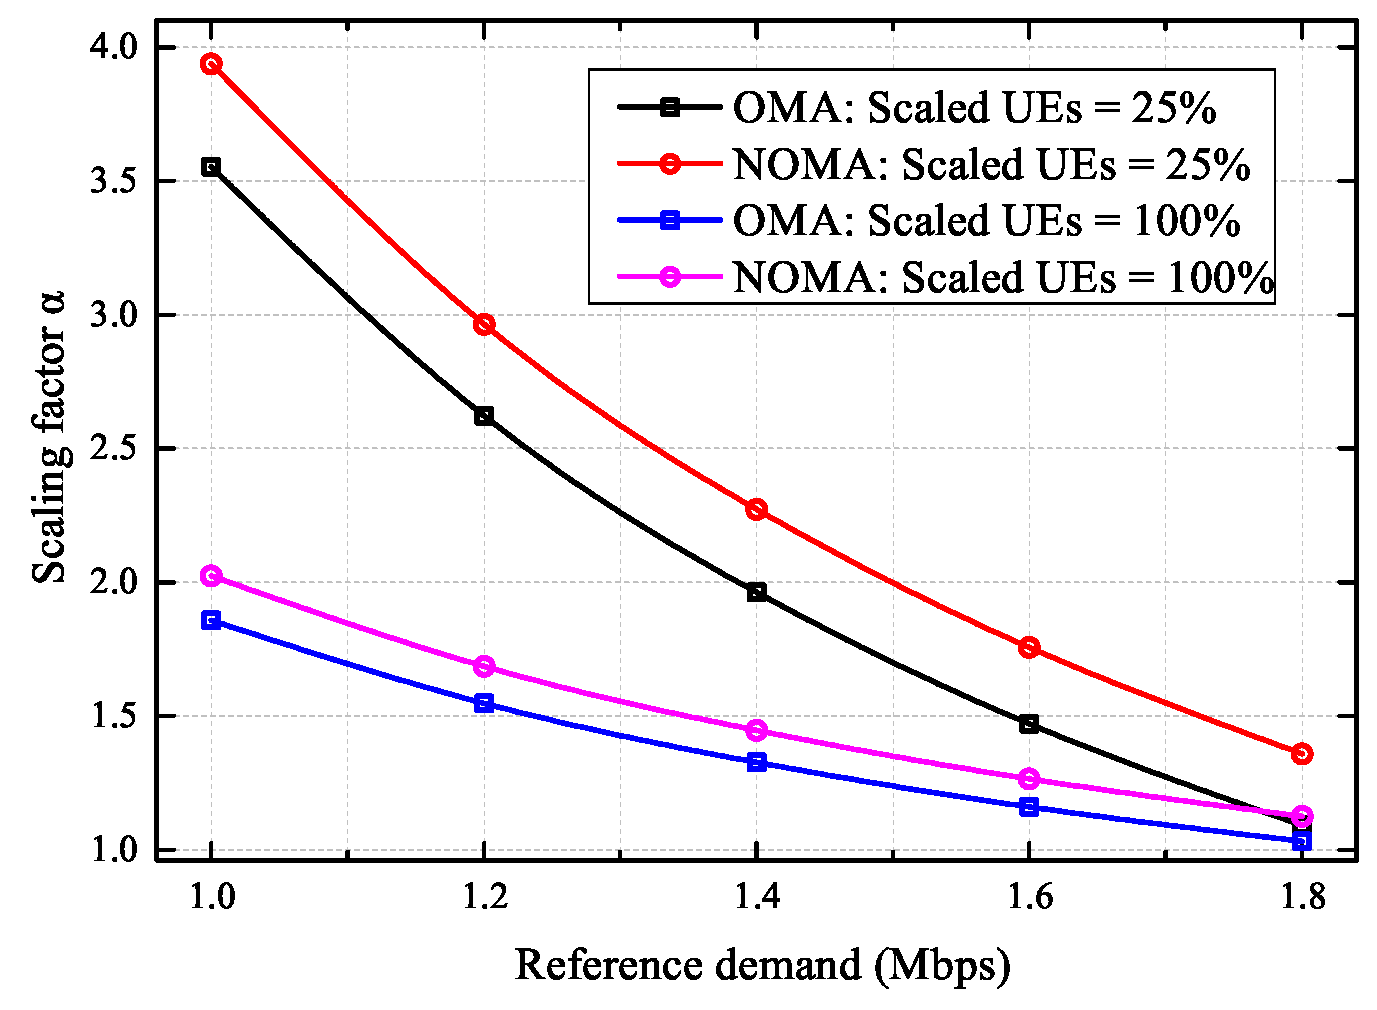
\includegraphics[width=0.5\textwidth, height=6.2cm]{1.eps}
\caption{This figure shows the scaling factor $\alpha$ in function of UE demand at NOMA and OMA with different percentage of scaled UEs}
\label{1}
\end{figure}

\begin{figure}
\centering
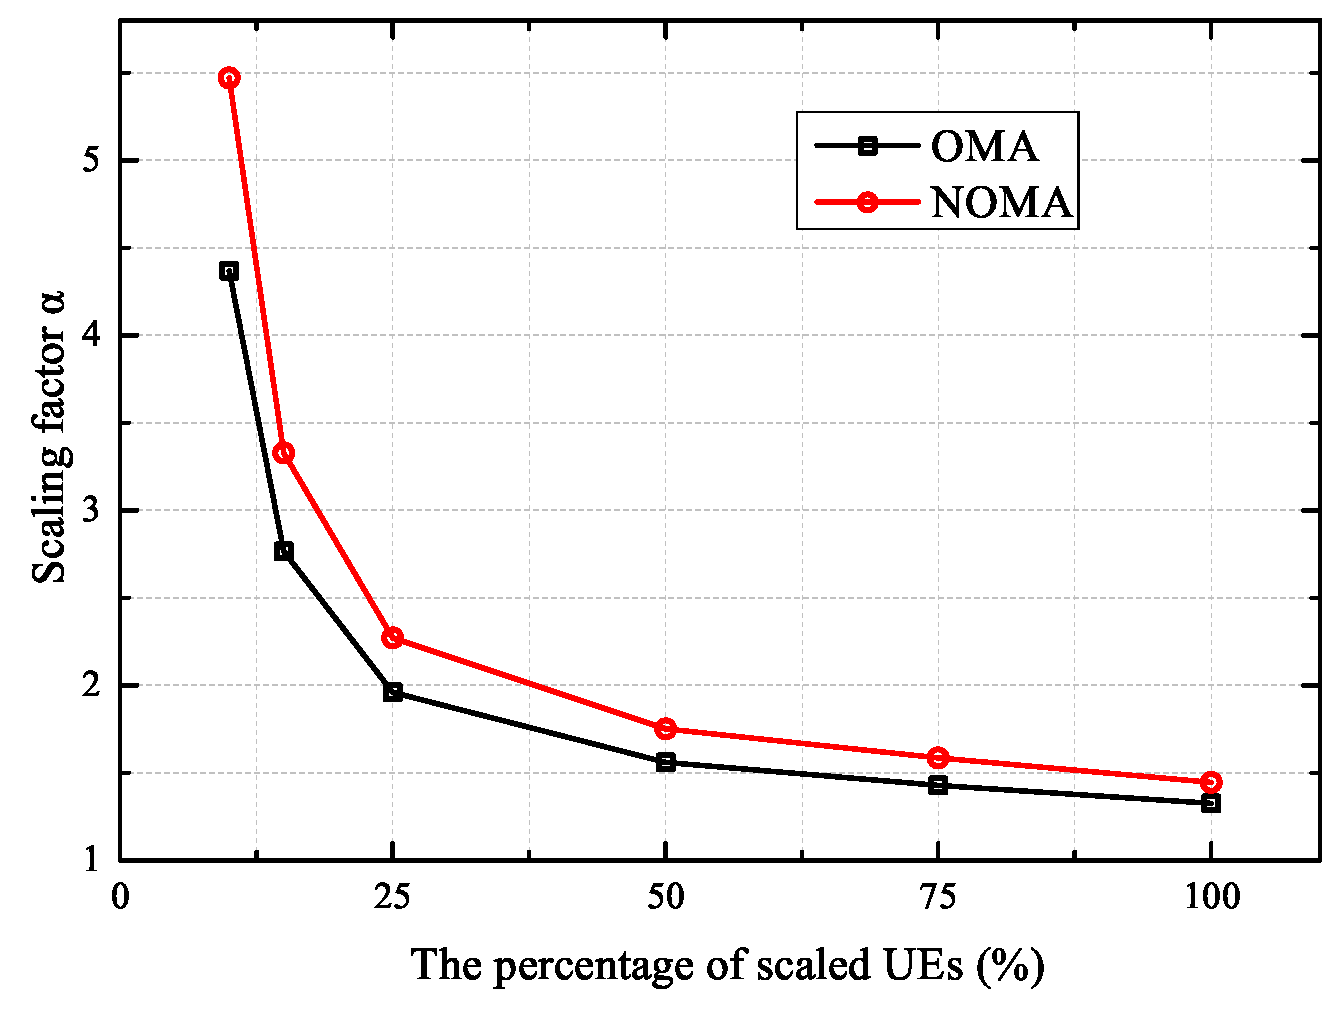
\includegraphics[width=0.5\textwidth, height=6.2cm]{2.eps}
\caption{This figure shows the scaling factor $\alpha$ in function of percentage of scaled UEs at NOMA and OMA with $d=0.07$.}
\label{2}
\end{figure}

\begin{figure}
\centering
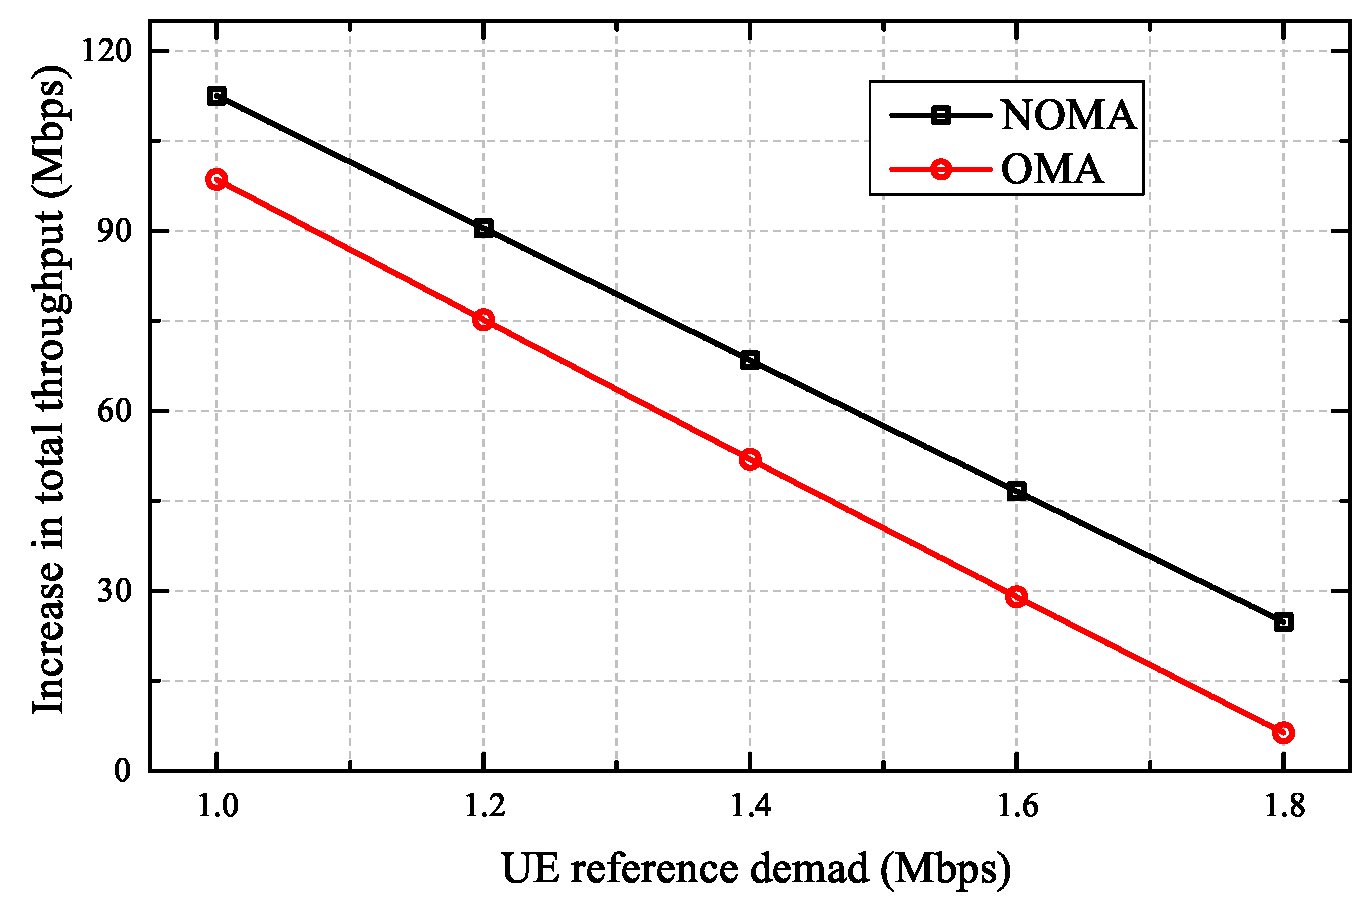
\includegraphics[width=0.5\textwidth, height=6.2cm]{3.eps}
\caption{This figure shows the increase of delivering data in function of UE demand at NOMA and OMA with $P\% = 25\%$.}
\label{3}
\end{figure}


%---------------------------------------------------------------------------------------------------------------------------------------------



\section{Conclusions}\label{Sec:Conclusions}

In this paper, we have studied a joint optimization problem of time-frequency resource allocation, UEs pairing and power split, aiming to improve the experience of edge UEs in multi-cell NOMA system. We have proposed an algorithmic framework for this problem, which can guarantee global optimality. Our numerical results have shown NOMA outperforms OMA in the field of improving the experience of edge UEs. 

%----------------------------------------------------------------------------------------------------------------------------
\begin{thebibliography}{99}

\bibitem{Do1}  T. N. Do, D. B. da Costa, T. Q. Duong and B. An, ``Improving the performance of cell-edge users in MISO-NOMA systems using TAS and SWIPT-based cooperative transmissions," {\em IEEE Transactions on Green Communications and Networking}, vol 2, no. 1, pp. 49-62, 2017.

\bibitem{Do2} T. N. Do, D. B. da Costa, T. Q. Duong and B. An, ``Improving the performance of cell-edge users in NOMA systems using cooperative relaying," {\em IEEE Transactions on Communications}, vol. 66, no. 5, pp. 1883-1901, 2018.

\bibitem{Guo} Q. Guo, C. W. Sung, Y. Chen, and C. S. Chen, ``Power control for coordinated NOMA downlink with cell-edge users", {\em IEEE Wireless Communications and Networking Conference (WCNC)}, 2018, pp. 1-6.

\bibitem{Pei} X. Pei, M. Wen and H. Yu, ``NOMA-based coordinated direct and relay system with multiple cell-edge users",  {\em IEEE International Workshop on Signal Processing Advances in Wireless Communications (SPAWC)}, 2019, pp. 1-5.

\bibitem{Ali} M. S. Ali, E. Hossain, A. Al-Dweik, and D. I. Kim, ``Downlink power allocation for CoMP-NOMA in
multi-cell networks," {\em IEEE Transactions on Communications}, vol. 66, no. 9, pp. 3982-3998, 2018. 

\bibitem{You1} L. You, D. Yuan, L. Lei, S. Sun, S. Chatzinotas, and B. Ottersten, ``Resource optimization with load coupling in multi-cell NOMA," {\em IEEE Transactions on Wireless Communications}, vol. 17, no.7, pp. 4735-4749, 2018.

\bibitem{You2} L. You and D. Yuan, ``A note on decoding order in optimizing multi-cell NOMA," {\em arXiv.org}, 2020. [Online]. Available: https://arxiv.org/abs/1909.08651.pdf

\bibitem{Ni} D. Ni, L. Hao, Q. T. Tran and X. Qian, ``Transmit power minimization for downlink multi-cell multi-carrier NOMA networks," {\em IEEE Communications Letters}, vol. 22, no. 12, pp. 2459-2462, 2018.

\bibitem{Lei} L. Lei, L. You, Y. Yang, D. Yuan, S. Chatzinotas and B. Ottersten, ``Load coupling and energy optimization in multi-cell and multi-carrier NOMA networks," {\em  IEEE Transactions on Vehicular Technology}, vol. 68, no. 11, pp.11323-11337, 2019.

\bibitem{Dai} L. Dai, B. Wang, Y. Yuan, S. Han, C. l. I, and Z. Wang, ``Non-orthogonal multiple access for 5G: solutions, challenges, opportunities, and future research trends," {\em IEEE Communications Magazine}, vol. 53, no. 9, pp. 74-81, 2015.

\bibitem{Islam} S. M. R. Islam, N. Avazov, O. A. Dobre, and K. S. Kwak, ``Power- domain non-orthogonal multiple access (NOMA) in 5G systems: Potentials and challenges," {\em IEEE Communications Surveys Tutorials}, vol. 19, no. 2, pp. 721-742, 2017.

\bibitem{41} D. Tse and P. Viswanath, {\em Fundamentals of Wireless Communication}. Cambridge university press, 2005.

\bibitem{48} ``IEC 80000-13:2008, quantities and units part 13: Information science and technology," International Electrotechnical Commission, 2008.

\bibitem{Yates} R. D. Yates, ``A framework for uplink power control in cellular radio
systems," {\em IEEE Journal on Selected Areas in Communications}, vol. 13,
no. 7, pp. 1341-1347, 1995.



\end{thebibliography}

\end{document}

